\section{Deployment View}\label{deployment-view}

\subsection{Requirements}\label{requirements}

\subsubsection{Operation System}\label{operation-system}

\paragraph{GPS\_Tracker}\label{gps_tracker-os}

The framework intended to run on Linux-based machines.

Tested OS:

\begin{itemize}
\tightlist
\item
  Debian 10/11
\item
  CentOS 7
\end{itemize}

\paragraph{GPS\_Android}\label{gps_android}

The version of Android must be 4.0+ (API level 14)

\paragraph{GPS\_Frontend}\label{gps_frontend}

The user should use one of the modern version of web-browser
HTML5-compatible:

\begin{itemize}
\tightlist
\item
  Google Chrome
\item
  Mozilla Firefox
\item
  Opera
\item
  Apple Safari
\end{itemize}

The browser should allow running JavaScript files.

\subsubsection{Hardware}\label{hardware}

There are no special hardware requirements.

\paragraph{GPS\_Android}\label{gps_android-hardware}

The Android phone must have Wi-Fi and GPS adapters.

\subsection{Configuration}\label{configuration}

GPS\_Tracker and GPS\_Frontend can be configured via a configuration
file provided in the projects or via the OS environment variables.

For the exact configuration instructions please check each of the
detailed project configuration sections.

\subsection{Deployment Cases}\label{deployment-cases}

Both GPS\_Tracker and GPS\_Frontend designed to be easily deployed.
Two possible two cases considered:

\begin{enumerate}
\def\labelenumi{\arabic{enumi}.}
\tightlist
\item
  Deployment on physical computers - the administrator should be aware of manually
  starting the software elements, or configure the OS properly (via
  systemd, InitV scripts, etc.)
\item
  Deployment in containers - the system provides Docker images
  description that can be started with \texttt{docker}, and a
  \texttt{docker-compose.yml} file to maintain the deployment phase more
  properly.
\end{enumerate}

Each system component may start on a separated machine if the conditions satisfied:

\begin{enumerate}
\def\labelenumi{\arabic{enumi}.}
\tightlist
\item
	Configuration files stay consistent across nodes running the system. 
\item
  	The nodes can reach each other on the network (NAT allowed, check for the ports if
  opened).
\end{enumerate}

\subsubsection{Deployment on physical computers}\label{bare-metal-deployment}

\begin{figure}[H]
\centering
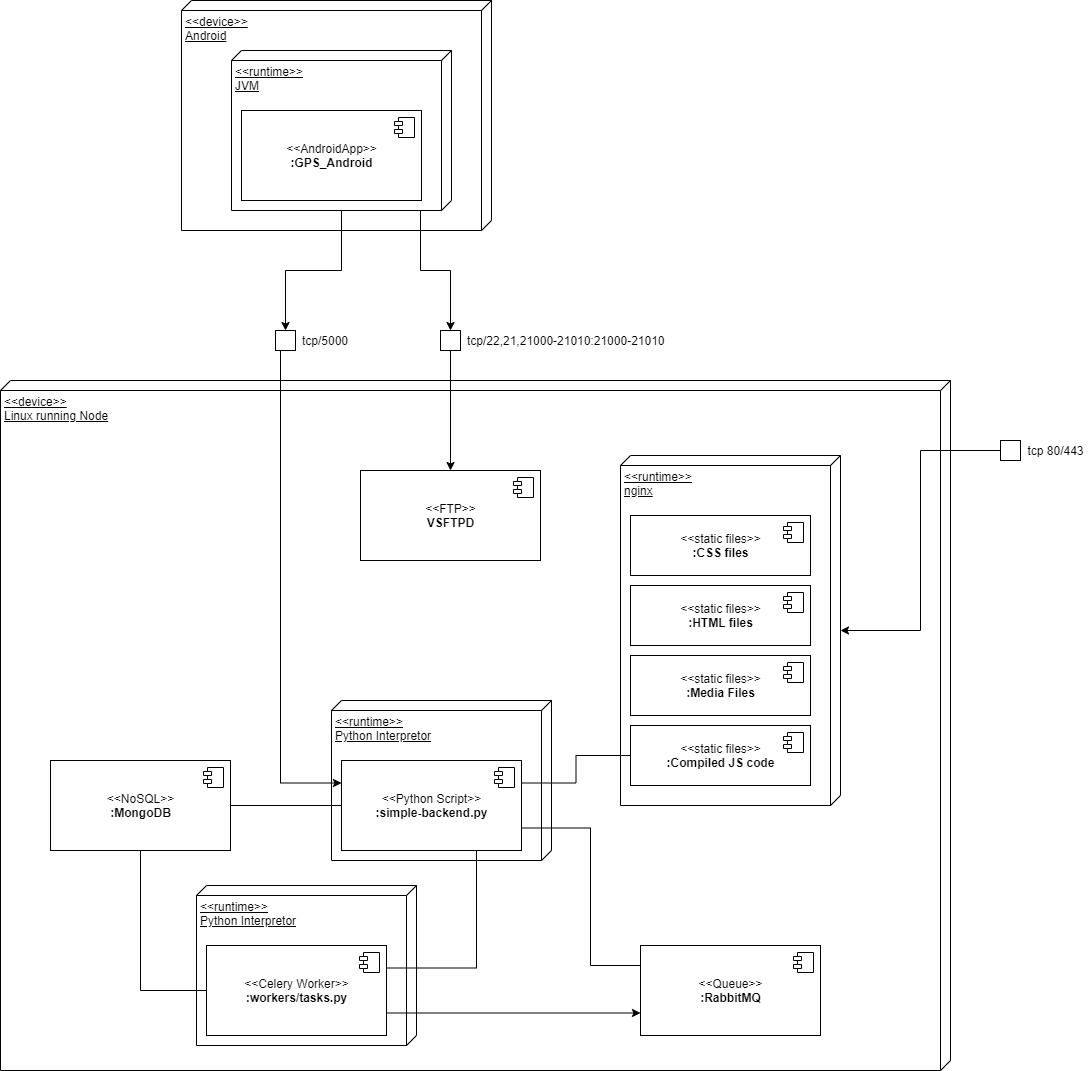
\includegraphics[width=\linewidth]{schemes/deployment/DeploymentDiagram-BareMetall.png}
\caption{Bare-Metal Deployment case}
\end{figure}

\subsubsection{Deployment in containers}\label{containerized-deployment}

\begin{figure}[H]
	\centering
	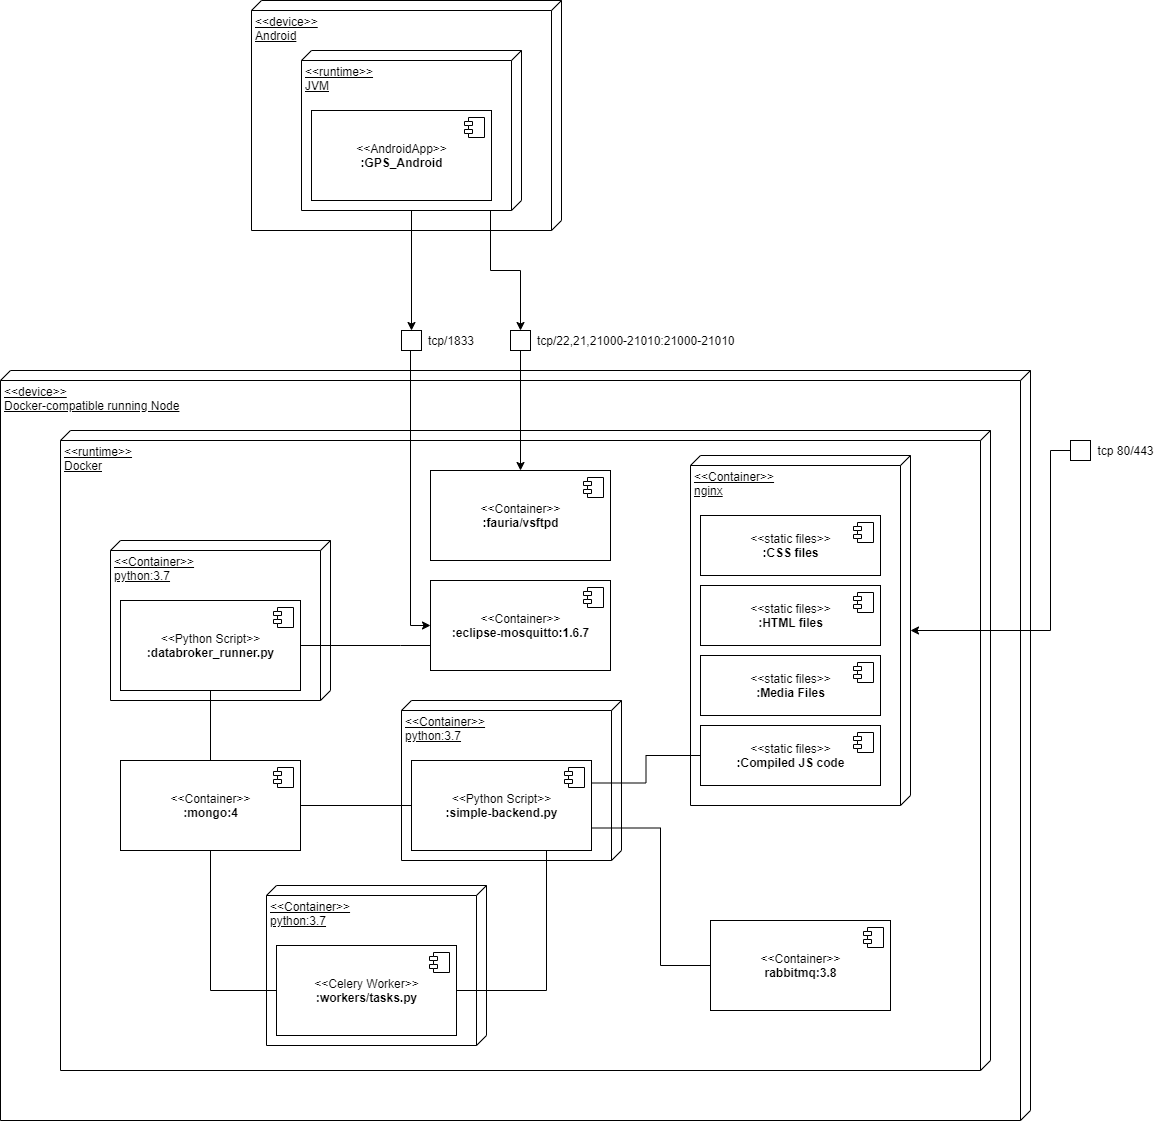
\includegraphics[width=\linewidth]{schemes/deployment/DeploymentDiagram-Containerized.png}
\caption{Docker Container Deployment case}
\end{figure}
